
\subsection*{1.}

3 \% représentent \(\dfrac{3}{100}\) des téléviseurs, soit \(0{,}03\).

On sait que sur les 3 \% de télés ayant un défaut de dalle, seuls 2 \% ont un défaut de condensateur, donc \(p_D(C) = \dfrac{2}{100} = 0{,}02\).

\subsection*{2.}

\begin{center}
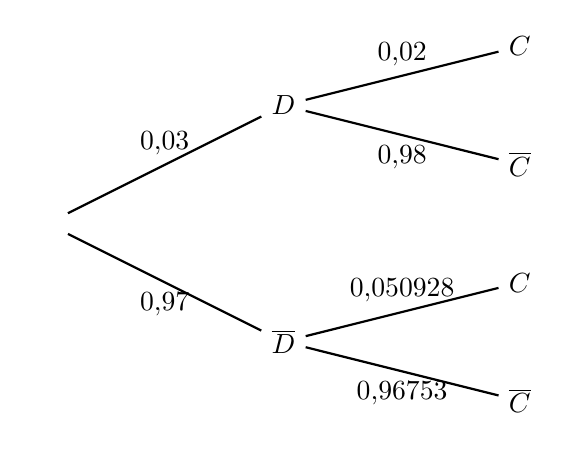
\begin{tikzpicture}[thick, scale=1.5]
\node (P_-1_0) at (-2,-1.5) {$\phantom{A}$};
\node (P_0_0) at (0,-0.5) {$D$};
\draw (P_-1_0) -- (P_0_0) node[midway, above] {$0{,}03$};
\node (P_1_0) at (2,-0) {$C$};
\draw (P_0_0) -- (P_1_0) node[midway, above] {$0{,}02$};
\node (P_1_1) at (2,-1) {$\overline{C}$};
\draw (P_0_0) -- (P_1_1) node[midway, below] {$0{,}98$};
\node (P_0_2) at (0,-2.5) {$\overline{D}$};
\draw (P_-1_0) -- (P_0_2) node[midway, below] {$0{,}97$};
\node (P_1_2) at (2,-2) {$C$};
\draw (P_0_2) -- (P_1_2) node[midway, above] {$0{,}050928$};
\node (P_1_3) at (2,-3) {$\overline{C}$};
\draw (P_0_2) -- (P_1_3) node[midway, below] {$0{,}96753$};
\end{tikzpicture}
\end{center}

\subsection*{3.}

\(p(D \cap C) = p(D) \times p_D(C) = 0{,}03 \times 0{,}02 = 0{,}0006.\)

\subsection*{4.}

Il faut calculer : \(p_C(D) = \dfrac{p(C \cap D)}{p(C)} = \dfrac{0{,}0006}{0{,}05} = 0{,}012\).

\subsection*{5.}

D'après la loi des probabilités totales, on a :
\[
p(C) = p(C \cap D) + p(C \cap \overline{D}),
\]
soit :
\[
0{,}05 = 0{,}0006 + p(C \cap \overline{D}) \iff p(C \cap \overline{D}) = 0{,}0494.
\]

\(\textit{Remarque : on peut compléter l'arbre ainsi}\). 

\[
p(C \cap \overline{D}) = \dfrac{p(\overline{D} \cap C)}{p(\overline{D})} \iff 0{,}0494 = \dfrac{p(\overline{D} \cap C)}{0{,}05},
\]  

d'où : \(p(\overline{D} \cap C) = 0{,}0494 \times 0{,}05 = 0{,}00247\).

Par conséquent : \(p(\overline{C} \cap \overline{C}) = 0{,}97 - 0{,}00247 = 0{,}96753\).

On termine avec : \(p_{\overline{D}}(C) = 0{,}050928\).

